\chapter{Xarxa Neuronal}
\section{Introducció}
En iniciar la part pràctica del treball vam decidir crear tres tipus de xarxes neuronals: una \nameref{sec:10}, una altra \nameref{sec:11} i, finalment, una \nameref{sec:12}.

En aquest capítol explicarem com vam elaborar cadascuna d’aquestes xarxes neuronals i, a més, compararem les dues formes de desenvolupament en una \nameref{sec:op}.

Per facilitar l’organització del treball, ens hem repartit les tasques: un membre de l’equip s’ha encarregat de la xarxa neuronal implementada amb llenguatge de programació Python, mentre que l’altre ha treballat una xarxa neuronal feta amb fulls de càlcul. Finalment, hem elaborat conjuntament la taula de comparació, intercanviant perspectives, i també hem treballat plegats la xarxa neuronal del cas real.

Les nostres pràctiques consisteixen en recopilar una sèrie de dades d'alumnes mitjançant una enquesta feta per nosalres amb la finalitat de crear una Xarxa neuronal que pugui predir la nota final de cada alumne. Les preguntes que hem fet en el formulari són sobre la matèria de matemàtiques i són les següents:
\begin{itemize}
 \item Realització de deures
 \item Hores d'estudis (semanal)
 \item Hores de section
 \item Interès en la matèria
 \item Nota del segon trimestre
 \item Nota del tercer trimestre
 \item Nota final
\end{itemize}
Com es pot veure, les preguntes d'aquest formulari estan relacionades amb el rendiment d'estudis dels alumnes, aquest formulari els hem enviat a alumnes de primer de bachillerat científic.


Després de les prediccions, compararem la xarxa neuronal feta amb python y la del full de càlcul i veurem quina de les dos té més precisió.

\section{Xarxa neuronal de regressió}\label{sec:op}
Una intel·ligència artificial és un camp molt extens i, dins d’aquest, les xarxes neuronals també representen una branca àmplia i complexa.
En el nostre context utilitzarem un tipus concret de xarxa neuronal per a la pràctica: les \textbf{xarxes neuronals de regressió}.

Una xarxa neuronal de regressió, a diferència d’una de classificació, té una sortida de tipus lineal que permet predir un valor numèric continu. Aquest tipus de xarxes requereixen un conjunt de dades prou extens i ben estructurat per poder aprendre les relacions entre les variables d’entrada i generar una estimació fiable.

A continuació es mostra un esquema representatiu d’una xarxa neuronal de regressió:

\begin{figure}[h!]
\centering
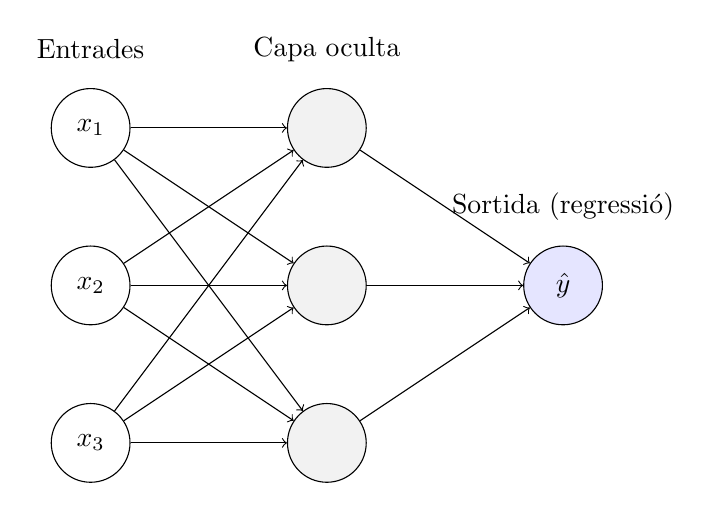
\begin{tikzpicture}[scale=1, transform shape]

% Input layer
\node[circle, draw, minimum size=1cm] (I1) at (0,2) {$x_1$};
\node[circle, draw, minimum size=1cm] (I2) at (0,0) {$x_2$};
\node[circle, draw, minimum size=1cm] (I3) at (0,-2) {$x_3$};

% Hidden layer
\node[circle, draw, fill=gray!10, minimum size=1cm] (H1) at (3,2) {};
\node[circle, draw, fill=gray!10, minimum size=1cm] (H2) at (3,0) {};
\node[circle, draw, fill=gray!10, minimum size=1cm] (H3) at (3,-2) {};

% Output layer
\node[circle, draw, fill=blue!10, minimum size=1cm] (O1) at (6,0) {$\hat{y}$};

% Connections input -> hidden
\foreach \i in {1,2,3}
  \foreach \h in {1,2,3}
    \draw[->] (I\i) -- (H\h);

% Connections hidden -> output
\foreach \h in {1,2,3}
  \draw[->] (H\h) -- (O1);

% Labels
\node at (0,3) {Entrades};
\node at (3,3) {Capa oculta};
\node at (6,1) {Sortida (regressió)};

\end{tikzpicture}
\caption{Esquema d’una xarxa neuronal de regressió}
\end{figure}

\section{Xarxa Neuronal amb llenguatge de programació}\label{sec:10}
En aquest apartat explicarem pas a pas de com vam crear el nostre xarxa neuronal de regressió.

\subsection{De celcius a fahrenheit}

Abans de començar a treballar amb la xarxa neuronal definitiu, vaig voler fer una més simple per tal de coneixer amb més profunditat de com funciona una xarxa neuronal de regressió; en aquest cas he escollit un transformador d'unitats de temperatura, de celcius (Unitat de temperatura basada en el punt de fusió de l'aigua) a fahrenheit (sistema d'unitat basada en el punt d'ebullició i solidificació de l'aigua). Per crear aquesta xarxa vaig escollir el Python com a llenguatge de programació, i el motiu esta explicat en l'apartat \ref{sec:4.4}.

\begin{comment}
\begin{figure}[H]
    \centering
    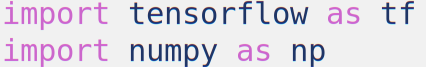
\includegraphics[width=0.5\textwidth]{./figures/1.png}
    \caption{biblioteques del Python}
\end{figure}
\end{comment}

Per començar a crear una xarxa neuronal lo primer que s'ha de fer es importar totes les biblioteques necessaries per el treball. En aquest cas he importat els biblioteques tensorflow i numpy, com podeu veure també he posat un as per transformar les nominacions de les biblioteques en abrevació.
\begin{itemize}
 \item \textbf{tensorflow: }
 \item \textbf{numpy: }
\end{itemize}














font(\href{https://www.youtube.com/watch?v=iX_on3VxZzkhttps://www.youtube.com/watch?v=iX_on3VxZzk}{Xarxa neuronal amb Python})


















\section{Xarxa Neuronal amb fulls de calculs}\label{sec:11}
En aquest apartat continuarem amb la xarxa neuranal de regressió però aquesta vegada utilizarem un full de calculs per fer-ho.
L'estructura que utilitzarem per aquesta pràctica serà la del perceptró.

\begin{figure}[H]
    \centering
    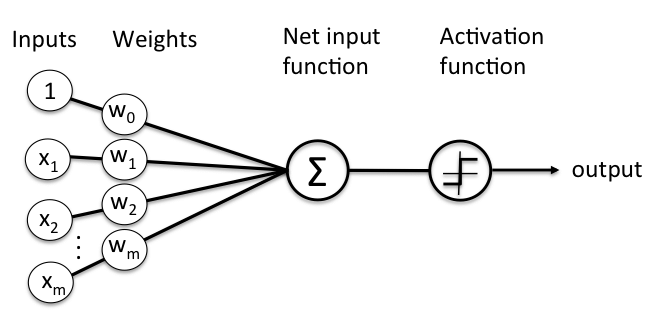
\includegraphics[width=0.5\textwidth]{./figures/perceptro.png}
    \caption{Estructura del perceptró}
\end{figure}

Un cop sabem quina estructura utilitzarem, començarem la pràctica ordenant les dades de cada alumne del formulari en el full de càlculs

\begin{figure}[H]
    \centering
    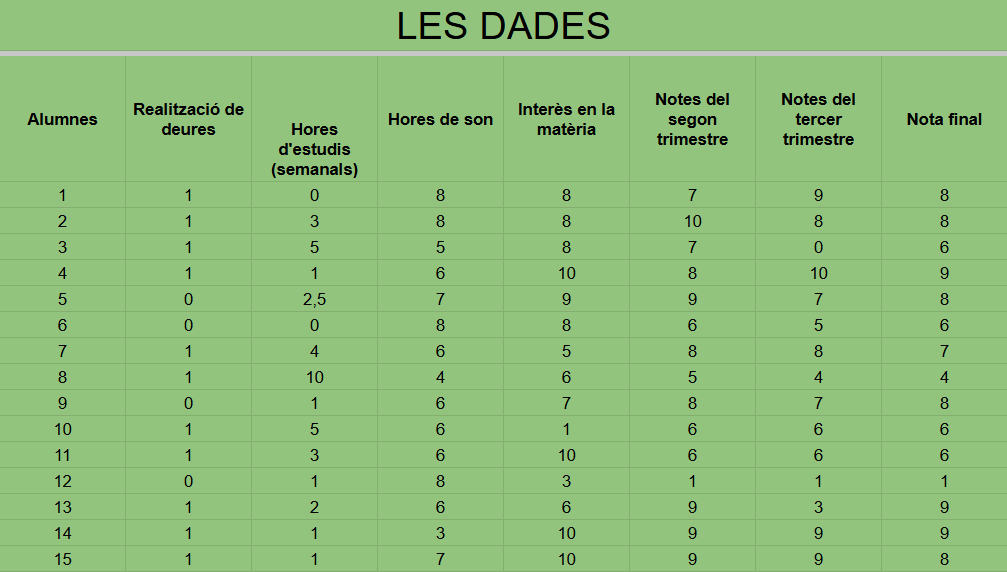
\includegraphics[width=0.5\textwidth]{./figures/Dades.png}
    \caption{Dades dels alumnes en el full de càlcul}
\end{figure}

Una vegada he ordenat tota la informació, he decidit representar els valors d'entrada d'una forma més senzilla d'entendre i curta, anomenantlos $xi$
\begin{itemize}
 \item \textbf Realització de deures: $x1$
 \item \textbf Hores d'estudis: $x2$
 \item \textbf Hores de son: $x3$
 \item \textbf Interès en la matèria: $x4$
 \item \textbf Notes del segon trimestre: $x5$
 \item \textbf Notes del tercer trimestre: $x6$
 \item \textbf Nota final: $y$
\end{itemize}

Aquestra representació queda així:

\begin{figure}[H]
    \centering
    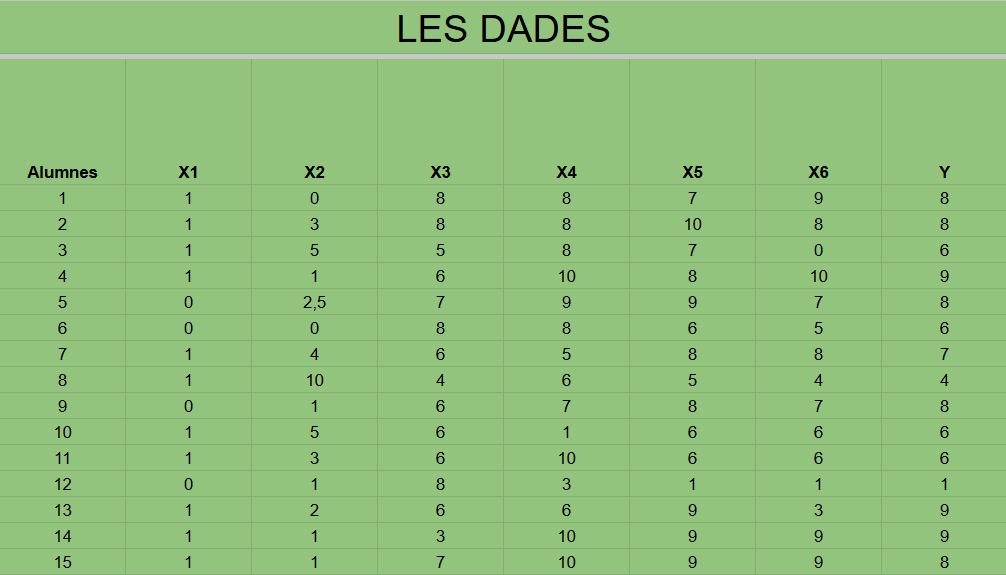
\includegraphics[width=0.5\textwidth]{./figures/Dades_resumides.png}
    \caption{Taula resumida}
\end{figure}

L'entrada de ``Realització de deures'' és una data binaria que nomès pot prendre valors 0 o 1.
\subsection{Normalització de dades}
Abans de continuar, és necessari explicar que és la normalització de dades.
La normalització de dades és una tècnica de procesament que consisteix en transformar dades de diferents escales a una escala comú, com per exemple del 0 al 1, aixó facilita la comparació i l'anàlisi de la xarxa neuronal i millora el seu rendiment. En el nostre cas, tenim dades binaries i dades ordinaries qe poden prendre qualsevol valor, aquest desequilibri afecta els càlculs posteriors si no es solucionen d'alguna manera.

Per aquesta raó, convertirem totes les dades en valors d'entre 0 i 1. Aquest procès implica calcular la miitjana de les dades i la desviació estàndar de cada variable. Per això utilitzant la fòrmula seguent:\\
$z = \frac{x - \mu}{\sigma}$\\

On:\\
$z$ És el valor normalitzat\\
$x$ És el valor original\\
$\mu$ És la mitjançan\\
$\sigma$ És la desviació estàndar\\

Aquests càlculs són fàcils d'obtenir amb les funcions que ens proporciona el full de càlcul.

\begin{figure}[H]
    \centering
    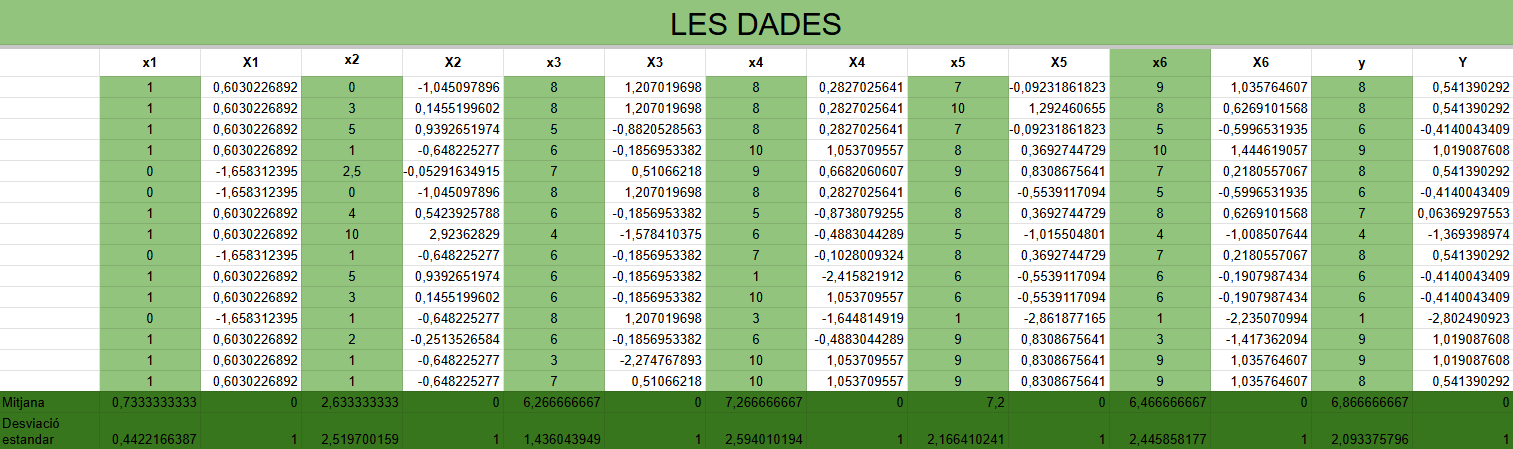
\includegraphics[width=0.5\textwidth]{./figures/Dades_normalitzades.png}
    \caption{Taula resumida}
\end{figure}

\section{Comparació entre una xarxa neurnal creada per un llenguatge de programació netre una de fulls de calculs}

\section{Xarxa Neuronal amb un cas real}\label{sec:12}
